\section{Создание демонстрационного приложения}
\subsection{Исследование примеров}
 Рассмотрим пример glass из пакета разработчика Optix. 
 Пример представляет собой класс GlassScene с рядом сопроводительных CUDA процедур и обработчиков запуска.
 Обработчиком запуска является процедура main:
 \begin{verbatim}
 int main(int argc, char* argv[])
{
  GLUTDisplay::init( argc, argv );

  bool adaptive_aa = true;  // Default to true for now
  bool green_glass = false;
  std::string obj_path;
  for ( int i = 1; i < argc; ++i ) {
    std::string arg( argv[i] );
    if ( arg == "--adaptive-off" || arg == "-A" ) {
      adaptive_aa = false;
    } else if ( arg == "--green" || arg == "-g" ) {
      green_glass = true;
    } else if ( arg == "--obj-path" || arg == "-o" ) {
      if ( i == argc-1 ) {
        printUsageAndExit( argv[0] );
      }
      obj_path = argv[++i];
    } else if ( arg == "--help" || arg == "-h" ) {
      printUsageAndExit( argv[0] );
    } else {
      std::cerr << "Unknown option: '" << arg << "'\n";
      printUsageAndExit( argv[0] );
    }
  }

  if( !GLUTDisplay::isBenchmark() ) printUsageAndExit( argv[0], false );

  if( obj_path.empty() ) {
    obj_path = std::string( sutilSamplesDir() ) + "/glass";
  }

  try {
    GlassScene scene( obj_path, adaptive_aa, green_glass );
    GLUTDisplay::setTextColor( make_float3( 0.2f ) );
    GLUTDisplay::setTextShadowColor( make_float3( 0.9f ) );
    GLUTDisplay::run( "GlassScene", &scene, adaptive_aa ? GLUTDisplay::CDProgressive : GLUTDisplay::CDNone );
  } catch( Exception& e ){
    sutilReportError( e.getErrorString().c_str() );
    exit(1);
  }

  return 0;
}
\end{verbatim}
Как  видно из исходного кода,  обработчик запуска создает объект класса GlassScene инициализирует его параметрами командной строки и передает его процессору запуска GLUTDisplay. Для корректной работы с GLUTDisplay класс GlassScene должен иметь следующие методы:
\begin{verbatim}
void   initScene( InitialCameraData& camera_data );
  void   trace( const RayGenCameraData& camera_data );
  void   doResize( unsigned int width, unsigned int depth );
  Buffer getOutputBuffer();
  bool keyPressed(unsigned char key, int x, int y);
\end{verbatim}
 InitScene создает объект сцены внутри контекста трассировки. 
 trace используется для построения изображения методом трассировки лучей.
 doResize производит необходимые изменения контекста для изменения получаемого изображения.
 getOutputBuffer создается выходной буфер, содержащий выходное изображение.
  keyPressed--- обработчик клавиш.
  Результат работы данного примера можно увидеть на рисунке \ref{glass}
\begin{figure}[h!]
\center{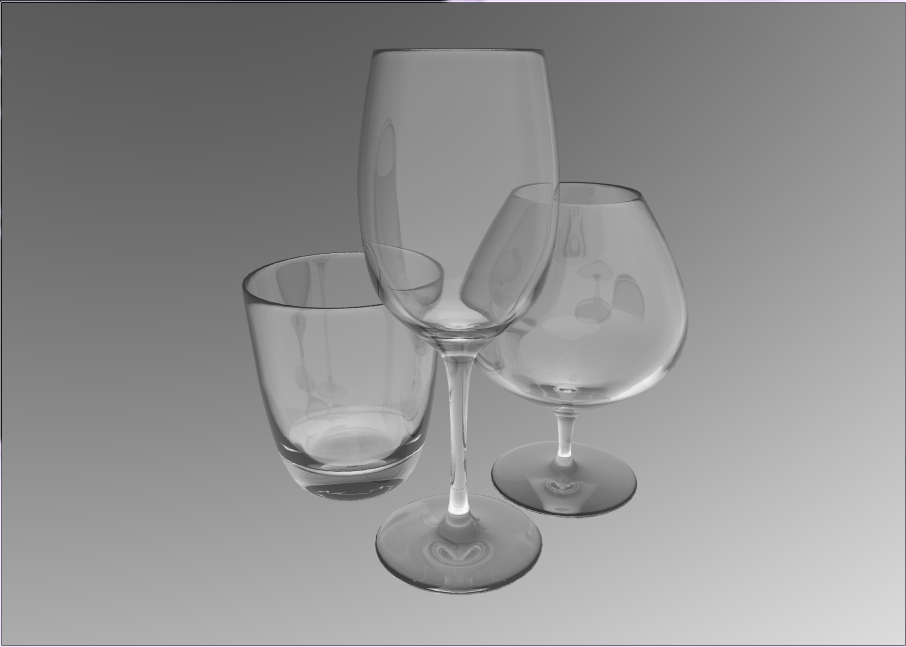
\includegraphics[width=0.5\linewidth]{glass.png}}
\caption{\small{Пример}}
\label{glass}
\end{figure}
 